\documentclass[conference]{IEEETran}

\usepackage[hmargin=.75in,vmargin=1in]{geometry}
\usepackage[american]{babel}
\usepackage[T1]{fontenc}
\usepackage{times}
\usepackage{caption}
\usepackage[]{algorithm2e}
\usepackage{textcomp}
\usepackage{epsfig,graphicx}
\usepackage{xcolor}
\usepackage{amsfonts,amsmath,amssymb}
\usepackage{fixltx2e} % Fixing numbering problem when using figure/table*
\usepackage{booktabs}
\usepackage{longtable}
\usepackage[utf8]{inputenc}
\usepackage{supertabular}
\usepackage{listings}
\usepackage{cite}
\usepackage{url}
\usepackage{float}

\definecolor{backcolour}{rgb}{0.95,0.95,0.92}
\lstset
{ %Formatting for code in appendix
    language=HTML,
    basicstyle=\footnotesize,
    numbers=left,
    stepnumber=1,
    numbersep=1pt,
    showstringspaces=false,
    tabsize=1,
    breaklines=true,
    breakatwhitespace=false,
    captionpos=b,
}



\columnsep 6mm  %%% DO NOT CHANGE THIS

% this will give huge title fonts in two rows
%\title{Parallel Hash Collision Search by Rho Method with Distinguished Points}

\title{\Large{\bf{WebChecker: An Epsilon Validation Language Plugin}}} % removed \bf \bfseries for authors


\author{\IEEEauthorblockN{Tebin M. Raouf}
\IEEEauthorblockA{Computer Science Dept.\\
College of Staten Island, CUNY\\
Staten Island, NY 11314, U.S.A.\\
tebin.raouf@cix.csi.cuny.edu}
\and
\IEEEauthorblockN{Dimitrios S. Kolovos}
\IEEEauthorblockA{Computer Science Dept.\\
University of York\\
Deramore Lane, York, YO10 5GH, UK.\\
dimitris.kolovos@york.ac.uk}
\and
\IEEEauthorblockN{Xiaowen Zhang}
\IEEEauthorblockA{Computer Science Dept.\\
College of Staten Island, CUNY\\
Staten Island, NY 11314, U.S.A.\\
xiaowen.zhang@csi.cuny.edu}}

\begin{document}
\maketitle

\begin{abstract}
WebChecker is an Epsilon Validation Language (EVL) plugin to validate static and dynamic Hyptertext Markup Language (HTML) pages that use frameworks such as Bootstrap by writing configurable EVL constraints. WebChecker is used for enforcing implicit rules of HTML and Cascading Style Sheet (CSS) frameworks. To show the effectiveness of the plugin, we choose Bootstrap, the world's most popular HTML, CSS, and JavaScript framework. The plugin comes with a list of EVL constraints for checking web pages built with Bootstrap. To support our argument, we present a concrete example with two solutions for enforcing implicit rules.  
\end{abstract}

\vspace{1em} \emph{\textbf{Keywords-\small Lint, Web Lint, EVL, Epsilon, HTML, Java, Bootstrap. }}

\section{Introduction}

In the current state of web development, there are many HTML and CSS frameworks that come with implicit rules. Such frameworks include Bootstrap \cite{bootstrap}, Materialize \cite{materialize}, Foundation \cite{foundation}, and uikit \cite{uikit}. These rules are developed for better use of such frameworks and best practices. Therefore, not following such rules impact appearances and framework features. Most of these frameworks are built to be responsive on different screen sizes such as large screens of personal computers and small screens of smart devices. To provide a consistent look and feel on all devices, it is important to follow such implicit rules. 


The Accessible Rich Internet Applications (ARIA) \cite{aria} specification introduces a handful number of rules for web pages in order to make them accessible for users with disabilities through assistive technologies such as screen readers. Such assistive technologies require web pages have certain attributes defined or enabled on HTML elements. Bootstrap, for example, provide default classes and ARIA attribute values throughout the framework for such technologies. Therefore, conforming to such rules make web pages available to a greater audience.

However, the caveat is to read frameworks' documentations carefully to capture such constraints and rules. This could be quite a tedious work and expensive. WebChecker is built to capture such rules so that users of these framework can easily check their web pages for the conformance of such rules. While WebChecker is built with HTML frameworks in mind, it could be easily used for web pages built without such frameworks. However, in this paper, we focus on the Bootstrap framework. Furthermore, WebChecker is able to check static and dynamic pages, which are generated by scripting languages such as PHP and JavaScript. 

The rest of the paper is structured as follows: Section II explains the problem and the current state of art solution and its limitations that motivated this project. In Section III, we explain the WebChecker plugin and we show our solution for the problem. In Section IV, we present a few sample implicit rules captured for the Bootstrap framework. We compare the current solution and our solution of the problem and its improvements in Section V. In Section VI, we discuss related work. Lastly, Section VII concludes the paper and outlines the future of the plugin and future work to enhance the plugin.  

\section{Background and Motivation}

Frameworks such as Bootstrap come with a handful number of implicit rules. While developing this project, we captured a couple of dozen rules for the Bootstrap framework. These rules should be followed in order to use the framework properly. These rules are created by the developers of such frameworks and explained in the framework’s documentation in a natural language. Users of such frameworks should carefully read the documentations in order to understand how to use the framework. This process can be quite long and tedious, expensive, and prone to errors. Given a set of rules, currently there is not a straightforward process to check if they are enforced against the HTML pages. At least, there is not an easy way that requires minimum effort and very little code. After collecting the rules, the current solution flow is:
1. Read and encode the HTML page. 
2. Translate each rule into a method. 
3. Check the rule against the HTML page.
4. Repeat 1-3 for every rule.
For example, in Bootstrap, any content should be under a \textit{<div>} element with class \textit{col}, which should be under a \textit{<div>} element with class \textit{row}, which should be under another \textit{<div>} element with class \textit{container}. The HTML code sample is at Listing \ref{lst:bge}.  

\begin{lstlisting}[language=HTML, caption=Bootstrap Grid Example, label={lst:bge}]
<!-- sample.html -->
<div class="container">
  <div class="row">
    <div class="col">
      Column One
    </div>
    <div class="col">
      Column Two
    </div>
    <div class="col">
      Column Three
    </div>
  </div>
</div>
\end{lstlisting}

To enforce this rule, the current state of the art solution is given in Listing \ref{lst:ebgr}. Since the plugin is written in Java, we choose it as our programming language of choice to implement this solution. However, any programming languages can be used. Some of which might take more or less coding. Listing \ref{lst:ebgr} shows, for enforcing the rule in Listing \ref{lst:bge}, the code can become lengthy and unreadable, which makes the logic confusing to reason about. It is also difficult to reuse and maintain this code since each rule has its own requirements and structure. Depending on the rules, it is likely to have more nested \textit{if statements}. Furthermore, the solution is not configurable. That is, it is difficult to make changes without breaking the code logic. This approach requires framework developers and users to spend quite some time to write similar code as Listing \ref{lst:ebgr} to enforce rules and constraints, and write documentations for such code.   

The above difficulties have motivated us to implement a plugin, WebChecker, for the Epsilon Validation Language (EVL) \cite{Kolovos2009}.  This plugin is designed for enforcing rules and constraints for any frameworks such as Bootstrap. With WebChecker, 1) a static or dynamic HTML file, 2) an HTML web page through its URL, and 3) a specific section of an HTML page can be checked for conformance. This plugin provides EVL constraint reusability across multiple projects and improves readability. Framework users and developers are able to focus on the rules and constraints. The next section explains WebChecker in more details.    

\begin{lstlisting}[language=Java, caption=Enforcing Bootstrap Grid Rule, label={lst:ebgr}]
		File input = new File("files/bootstrap/newCheck.html");
		try {
			Document doc = Jsoup.parse(input, "UTF-8");
			Elements elements = doc.getElementsByTag("div");
			for (Element element : elements) {
				if (element.hasClass("col-sm-4")) {					
					if (!element.parent().hasClass("row")) {
						System.out.println("A div element with class col should have a parent element with class row");
					} else {
						if (!element.parent().parent().hasClass("container")) {
							System.out.println("A div element with class col should have a parent element with class row, which has a parent with class container.");
						}
					}
				}
			}		
		} catch (IOException e) {
			e.printStackTrace();
		}
\end{lstlisting}


\section{WebChecker Plugin}
Epsilon Validation Language (EVL) \cite{Kolovos2009} is one of the languages of Epsilon \cite{EpsilonProject}, which is an Eclipse project that provides languages for model managements such as model validation, model transformation, code generation, pattern matching, model merging and etc. In the context of WebChecker, a model is an HTML page or a section of the page. WebChecker implements Epsilon Model Connectivity (EMC) layer that provides an interface, IModel, to capture the HTML model and EVL constraint file. The two main classes implemented by the plugin are \textit{WebCheckerModel} and \textit{WebCheckerPropertyGetter} while the other classes are provided by Epsilon. Figure \ref{fig:webcheckerclass} shows this relation. Furthermore, EVL users can use the features of WebChecker without setting up a new development workflow or installing new software.   


\begin{figure}
  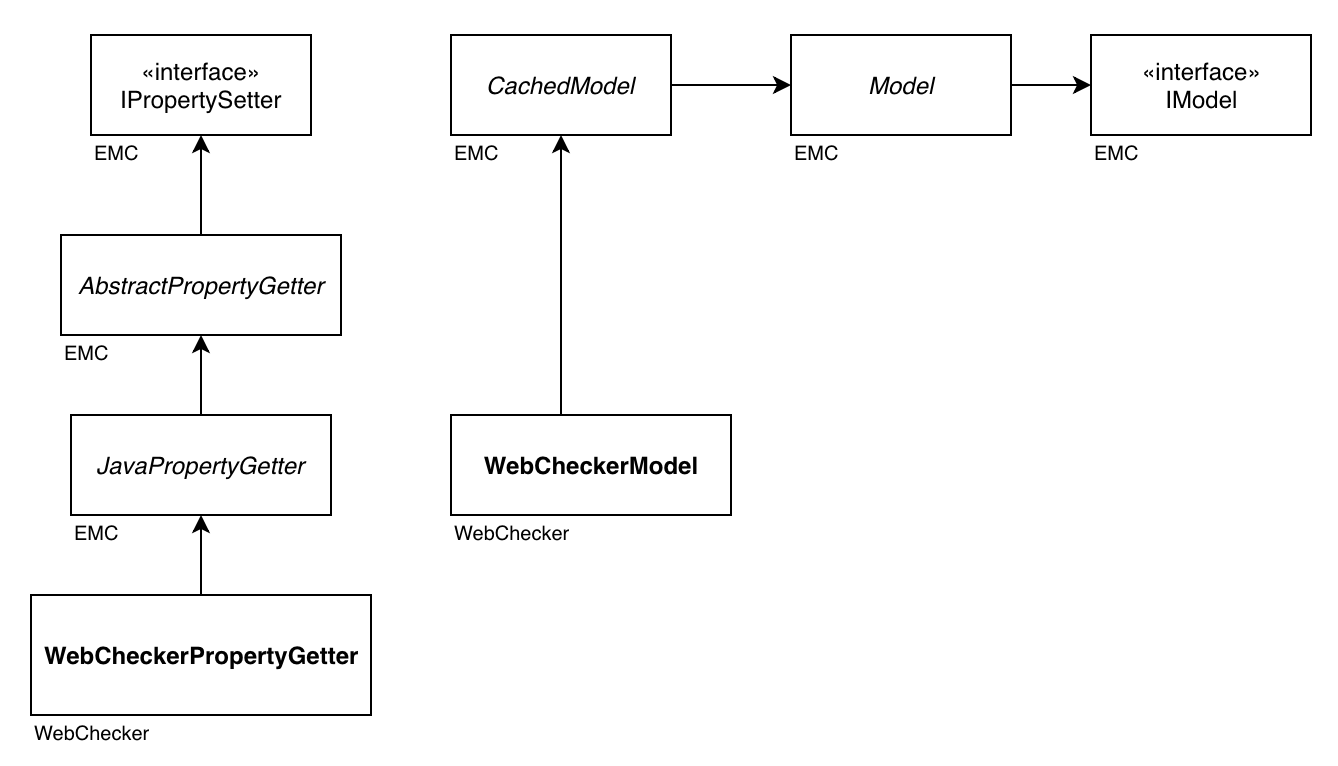
\includegraphics[width=\linewidth]{figures/webchecker-class.png}
  \caption{WebChecker and Partial EMC Diagram}
  \label{fig:webcheckerclass}
\end{figure}

\subsection{WebChecker}
The WebChecker flow, after collecting the constraints, is: 
1) Write an EVL constraint.
2) Choose the HTML source (i.e. an HTML file, URL, or section of HTML).
These two steps are modular and readable. Listing \ref{lst:webcheckerSolution} is an example of EVL file, which shows the solution for Listing \ref{lst:bge}. 

WebChecker follows the \textit{separation of concern}\footnote{According to Wikipedia \textit{separation of concern} is as a design principle for separating a computer program into distinct sections.} principle with writing minimum code. In particular, there is an EVL source file and an HTML source, which could be an HTML file content or its URL. The EVL file that contains the constraints such as Listing \ref{lst:webcheckerSolution} is run against the HTML source. Listing \ref{lst:linkEVLAndHTML} shows this connection. Line 10 and 11 of Listing \ref{lst:linkEVLAndHTML} set the HTML and EVL source respectively. Moreover, line 15 of Listing \ref{lst:linkEVLAndHTML} shows how to handle errors returned from the EVL constraints. This way the framework user and developer can only focus on constraints that do not satisfy.   

\begin{lstlisting}[language=Java, caption=Checking an EVL file against an HTML source file, label={lst:linkEVLAndHTML}]
 	//sample.java    
		//Step 1: Get the source to be validated
		String html = "files/bootstrap/newCheck.html";
		
		//Step 2: Write your validation using Epsilon Validation Language
		String evl = "files/bootstrap/newCheck.evl";
		
		//Step 3: Check the validation against the html in step 1
		WebChecker checker = new WebChecker();
		checker.setSource(html);
		checker.setValidation(evl);
		checker.check();
		
		//Step 4: Check the result
		List<String> errors = checker.errors();


\end{lstlisting}

\subsection{WebChecker EVL Structure}
The WebChecker EVL structure follows the same EVL structure \cite{Kolovos2009}. However, here we only explain the current syntax used by WebChecker. 


\begin{lstlisting}[language=Java, caption=Enforcing Bootstrap Grid Rule by Using WebChecker, label={lst:webcheckerSolution}]
//sample.evl
context t_div { 
    constraint DivWithColHasRowParent {
        guard : self.class.includes("col-*")
        check : self.parent.hasClass("row") and self.parent.is("div")
        message : "A <div> element with class col should have a parent <div> element with class row."
    }
    constraint DivWithRowHasContainerParent {
        guard : self.class.includes("row")
        check : self.parent.hasClass("container") and self.parent.is("div")
        message : "A <div> element with class col should have a parent <div> element with class row."
    }
}

\end{lstlisting}

\begin{itemize}
\item \textit{Context}: an EVL file could have one or more contexts. To capture an HTML element, a context should start with \textit{t\_}, for \textit{type}, followed by the name of the HTML element such as \textit{t\_div}, \textit{t\_picture}, \textit{t\_section}, \textit{t\_button}, and etc.
\item \textit{Constraint}: each \textit{Context} could have one or more constraints. A \textit{constraint} has a name that is used to differentiate each constraint from each other. While the constraint name does not matter, we suggest having a name that identifies the rule. Each \textit{constraint} has three blocks \textit{guard}, \textit{check}, and \textit{message}. Optionally, an EVL constraint could have a \textit{fix} section, where the model is fixed if the constraint does not satisfy. Currently, WebChecker does not utilize this feature. Section VI explains future enhancements to WebChecker where the \textit{fix} block is explained. 
\item \textit{guard}: this block captures a specific section of the context for checking. \textit{guard} must return a boolean value. If true, the \textit{check} block is executed. The \textit{guard} block accepts compound boolean statements by using \textit{and} and \textit{or}.      
\end{itemize}
\begin{itemize}
\item \textit{check}: after the \textit{guard} block is satisfied, this block is executed to \textit{check} if the constraint is satisfied. Expressions in this block must return a boolean value. If the expression returns true, the constraint is satisfied and hence the \textit{message} block is not executed. Similarly as the \textit{guard} block, this block accepts compound boolean statements.
\item \textit{message}: this block returns a message if the constraint is not satisfied. WebChecker provides a convenient method to capture all unsatified constraints' messages shown in Line 15 of Listing \ref{lst:webcheckerSolution}.  
\end{itemize}

\section{Sample Bootstrap Implicit Rules}
In this section, we show and explain a few implicit rules captured for the Bootstrap framework. The following are randomly chosen and more rules can be accessed from the plugin repository \footnote{https://github.com/tebinraouf/webchecker} For brevity, we do not show the actual EVL syntax.
  
\begin{itemize}
\item \textit{ScreenReaderButton}: this constraint captures buttons with class \textit{close} and validates if the \textit{<button>} element has the \textit{aria-label} attribute defined for assistive technologies.
\item \textit{AlertLinkInDivAlert}: this constraint captures \textit{<a>} elements with class \textit{alert-link} and validates if the parent element includes \textit{alert} and \textit{alert-*} classes. The asterisk (*) is a wild card such as \textit{alert-success} or \textit{alert-danger} and etc.
\item \textit{BtnGroupToggle}: this constraint captures \textit{<div>} elements with class \textit{btn-group-toggle} and checks if its \textit{data-toggle} attribute is defined and its value is equal to \textit{buttons}.
\end{itemize}

\section{Improvements over Current Solution}
As shown from the example above, WebChecker is built to be easy, modular, readable, and configurable. These features address and solve most of the challenges developers face while using a program analyzer as studied by Microsoft researches \cite{christakis16}. WebChecker, specifically, offers custom warning messages, platform independency, static and dynamic page analysis, and easy integration into development workflow. Importantly, it is left to the developer to check HTML pages against any set of EVL constraints, which makes WebChecker stand out among other validators that have default un-configurable rules.    

Furthermore, WebChecker provides an abstract class, \textit{WebChecker},  to interact with the underlying model. While users can (should) use the \textit{WebChecker} class, they are not restricted to use the \textit{WebCheckerModel} class, which implements CachedModel of EMC. While \textit{WebCheckerModel} requires background knowledge on Epsilon, it could be very powerful and configurable. The WebChecker abstract class allows a user to focus on the constraints rather than writing code, which saves time and resources. WebChecker modularity allows it to be reusable and extensible. If new framework rules are in place, WebChecker can be modified or extended to support such rules. 

Code written like Listing \ref{lst:ebgr} is prone to errors and confusing, which makes the code unreadable to none technical stakeholders such as managers and web designers. Also, as stated above the code in Listing  \ref{lst:ebgr}  is written in Java. It is likely the developer uses a language that their workflow uses for validation such as JavaScript, PHP, C\#, Python and etc. This makes it difficult to use the code in other development environment that uses different programming languages and technology stack. In contrast, WebChecker's EVL constraints are easy to reason about and independent of the development environment. That is, as long as the source HTML is given to WebChecker, how the HTML is generated does not matter. 

Line 3 of Listing \ref{lst:ebgr} uses \textit{jsoup: Java HTML Parser}\cite{jsoup} library to parse the HTML file into \textit{jsoup's Element} objects. While \textit{jsoup} is very powerful, it is irrelevant in this context because a user does not need to learn a new library that is unrelated to a validation task. How the HTML file is parsed into objects should be done internally. WebChecker abstracts this by having the user only set the source of the HTML file as shown in Line 10 of Listing \ref{lst:linkEVLAndHTML}.           


The \textit{for-loop} and the \textit{try-catch} blocks in Listing \ref{lst:ebgr} are the least important to the user. WebChecker improves this by introducing a clear readable structure as explained in the WebChecker EVL Structure section above. Table \ref{table:compareWebChecker} shows a side by side comparison of WebChecker with other current validators, purely based on our research and experiment.    
 
\begin{table}[H]
\begin{tabular}{|l|c|c|}
\hline
\textbf{Features}   	 & \textbf{WebChecker} 	& \textbf{Other} \\ \hline
Reusability 	 & \checkmark   	&       \\ \hline
Configurable      & \checkmark        			&       \\ \hline
Extensible        &    \checkmark        			&       \\ \hline
Platform Independence        &    \checkmark        			&       \\ \hline
Minimum Coding        &    \checkmark        			&       \\ \hline	
Task Specific       &    \checkmark        			&       \\ \hline
Dynamic Page Analysis       &    \checkmark        			&       \\ \hline
Static Page Analysis       &    \checkmark        			& \checkmark      \\ \hline	
\end{tabular}
\caption{WebChecker Plugin Compared to Other Tools}
\label{table:compareWebChecker}
\end{table}


\section{Related Work}
Bootlint \cite{bootlint} is a Bootstrap specific linter for checking common HTML mistakes in web pages built in a vanilla way; that is, pages where default Bootstrap classes are used. Bootlint uses JavaScript to check for Bootstrap rule conformance, which is not configurable. The source code of Bootlint, which is in the \textit{bootlint.js}\footnote{https://github.com/twbs/bootlint/blob/master/src/bootlint.js} file of the Bootlint project, is much lengthier than the code in Listing 2. This validates our points on the current limitations of the current solution as explained above. 

Policheck is Microsoft's internal tool that checks codes, comments, and contents including web pages. For example, it can check if a web page contains inappropriate content or its style matches best practices and guidelines \cite{christakis16}.

ESLint \cite{eslint} is a static JavaScript analysis linting utility written in JavaScript to enforce coding styles through pluggable rules. With ESLint, developers can analyze JavaScript code by using default rules or creating new rules without running the JavaScript code. ESLint requires a configuration file in JavaScript Object Notation (JSON), YAML (YAML Ain't Markup Language) or JavaScript. Most importantly, the configuration file includes the source of the rule file, which is a JavaScript file that has the implementation of the rule. While ESLint is powerful and popular, the JavaScript code for each rule is not reusable.    
 


\section{Conclusion and Future Work}

In this paper, we have proposed a new plugin for the Epsilon Validation Language with a concrete example. We identified the current solution developers use to check web pages for framework rule conformance, and compared our solution with the improvements it brings. 

We believe that with web pages being ubiquitous, there will be more frameworks with implicit rules and less detailed documentations. If developers of these frameworks have a tool such as WebChecker, they can write exhaustive lists without providing much documentations since EVL constraints are easily readable and close to a natural language. 

Further research on the topic includes extending WebChecker to support fixes when a constraint does not satisfy, evaluating other framework rules and capturing such implicit rules, providing WebChecker through popular text editors, validating web pages online, project-wise validation, and developing a domain specific language for capturing and enforcing such rules that is easy to integrate with a development workflow.

\bibliographystyle{ieeetr}
\bibliography{References} 

\end{document}
